\documentclass[30pt, b2paper, landscape]{tikzposter}
\usepackage[utf8]{inputenc}
\usepackage[brazil]{babel}
\usepackage{indentfirst}
\usepackage{graphicx}
\usepackage{subfig}
\usepackage{float}
\usepackage{hyperref}
\usepackage{blindtext}
\usepackage{dirtytalk}
\newcommand{\proj}{DELPo }
\newcommand{\nehilp}{Nucleo de apoio à pesquisa em Etimologia e História da Língua Portuguesa (NEHiLP) }


\author{Andre Luiz Abdalla Silveira ($8030353$) \\ Marco Dimas Gubitoso (Orientador)}
\title{\proj--- Dicionário Etmológico da Lígua Portuguesa}
\date{\today}
\institute{Universidade de São Paulo --- Instituto de Matemática e Estatística}

\usetheme{Envelope}

\begin{document}
  \maketitle

  \begin{columns}
    \column{0.2}

    \block{Do que se trata?}{
    O \proj se trata de um portal onde pesquisadores podem investigar as origens de um verbete, podendo conhecer
    sua evolução temporal. O \proj é um projeto do \nehilp criado pelo professor Mario Viario em 2012. \\

    Além do \texttt{moedor} que é a funcionalidade principal do sistema, há também o multiplasmador que é toma
    uma palavra em latim vulgar e presume sua evolução em etapas até se tornar familiar ao que observamos nos dias
    de hoje. Há também ferramentas que permitem observar a frequência de determinada ocorrência ao passar dos anos.
    }

    \block{Objetivos}{
    \begin{itemize}
      \item Fazer um sistema de duas camadas (interior e exterior) que provesse as funcionalidades já existentes
      e que pudesse escalar o bastante para confortar outras tantas
      \begin{itemize}
        \item A camada interior (Back end) é onde se encontra a mior parte das regras de negócio -- implementada
        em Ruby on Rails
        \item A camada externa (Front end) é a de apresentação. É a interface de comunicação entre o usuário e a
        camada interior
      \end{itemize}
      \item Refatorar o código do moedor, removendo os \say{cheiros} (problemas) do código
      \item Usar padrões de design na medida do possível
      \item Garantir que o código resultante seja o melhor possível para que quaisquer desenvolvedores possam
      escalar as duas camadas da aplicação
    \end{itemize}
    }

    \column{0.6}

    \block{Back End -- Ruby on Rails}{
    Ruby on Rails é um framework em Ruby. Não se trata de algo revolucionário, visto que usa algumas ferramentas
    já validadas como o \emph{ActiveRecord} (uma biblioteca que transforma entidades e relacionamentos em objetos),
    e o paradigma MVC (model - view - controller). Provavelmete o que possui o maior potenncial é a possibilidade
    de criar uma aplicação com operações CRUD (create - read- update - delete) com relativamente pouco esforço \\

    A aplicação feita em Ruby on Rails era a única camada do \proj até o andamento deste projeto. No começo do
    ano, haviam controladores, modelos, mas não havia testes e as visualizações não apresentavam estilização
    alguma. \\

    A primeira coisa a fazer foi conhecer a implementação atual para saber como tudo funcionava. Tudo funcionava,
    mas algumas refatorações como a da figura abaixo eram necessárias. Os dois trechos de código fazem a mesma coisa,
    a diferença é que na segunda imagem, o código está mais organizado

    \begin{tikzfigure}
      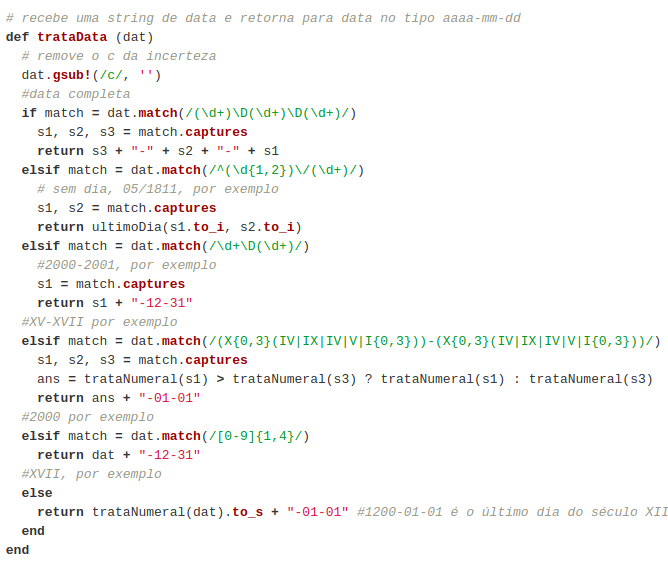
\includegraphics[width=.15\textwidth]{../figuras/antes.png}
      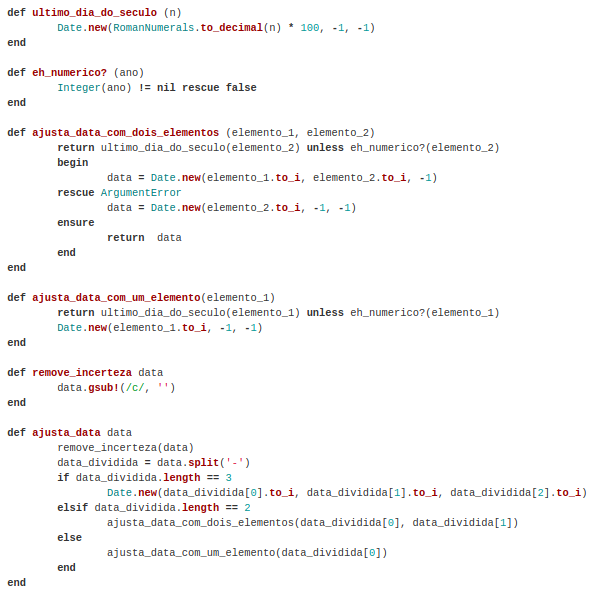
\includegraphics[width=.12\textwidth]{../figuras/depois.png}
    \end{tikzfigure}

    Além disso, decidido por usar outro framework para fazer as visualizações, transformei a aplicação Rails em
    uma API (Application Program Interface) para aproveitar tudo o que o Rails tem a oferecer. A partir dessa
    decisão, e de necessidades consequentes, gemas foram adotadas e abandonadas, mantendo as funcionalidades,
    melhorando a qualidade do código (não estava ruim, mas alguns detalhes que passaram batido como aproveitar-se
    do ActiveRecord foram reparados).
    }

    \block{Front End -- Nuxt.js}{
      Nuxt.js é um framework construído sobre outro: o Vue.js, que pode ser usado pra outras finalidades além da
      construção de páginas web. De uma forma similar ao Rails, que junta o que há de mais relevante no universo Ruby,
      o Nuxt é uma aplicação em Vue, só que com plug-ins essenciais como Vue Router (controla as rotas) e Vuex (onde
      ficam as \say{variáveis globais}) já vêm imbutidos na aplicação de modo que não se faz necessário lidar com esse
      e tantos outros detalhes. Além disso, Nuxt também otimiza o carregamento dos elementos da página, possibilitando
      uma melhor experiência de usuário. \\

      O motivo principal pelo que se decidiu pelo uso do Nuxt ao invés do sistema nativo do Rails é o fato do último
      ser menos flexível em seu desenvolvimento. O desenvolvimento em Rails prefere convenções ao invés de configurações.
      Enquanto isso poupa algum trabalho a configurar suas preferências, por outro lado, prende o desenvolvedor a fazer
      as coisas do modo que \say{reza a cartilha} do framework, podendo muitas vezes dar terríveis dores de cabeça em
      quem se atreve a descomprir as convenções. Abaixo, a página principal da plataforma. \\

      \begin{tikzfigure}
        \centering
        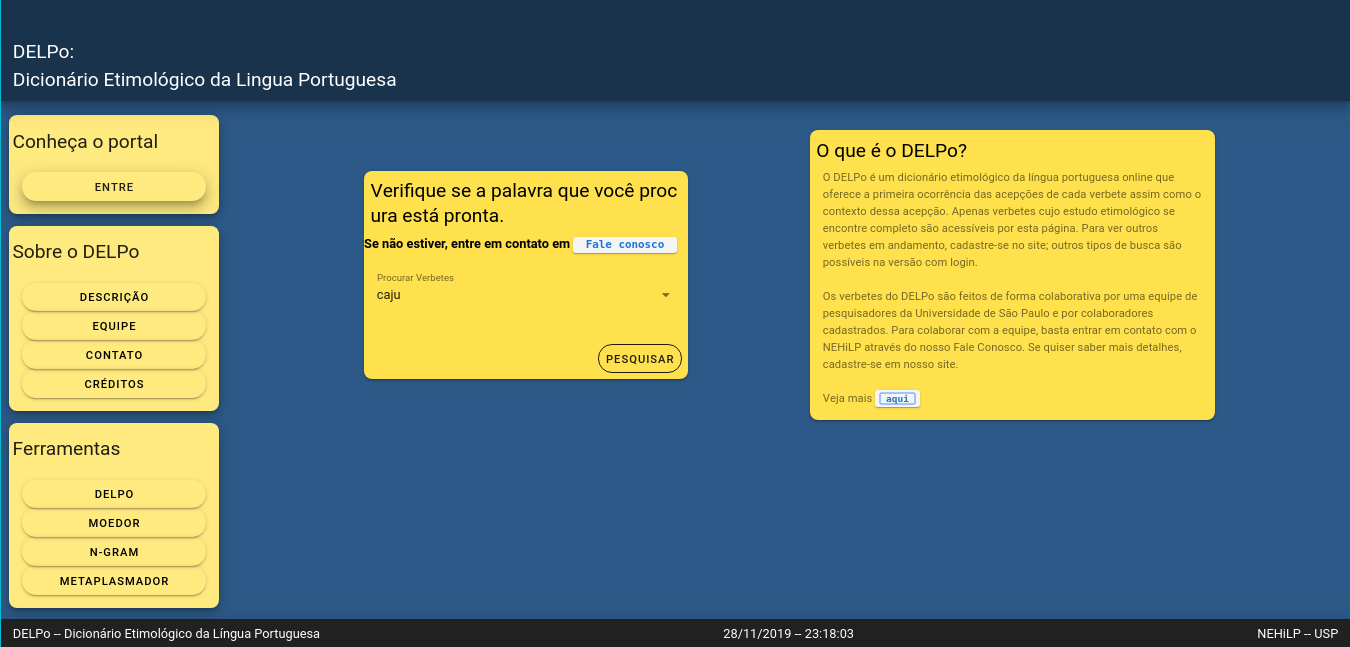
\includegraphics[width=.15\textwidth]{../figuras/home.png}
      \end{tikzfigure}
    }

    \column{0.2}

    \block{Reflexão Importante}{
      Durante o desenvolvimento dessa aplicação, aprendi muitas coisas, e a principal é como equilibrar o ímpeto
      quase perfeccionista de fazer sempre o melhor código possível. Houveram ocaisões em que me encontrei bloqueado a
      pensar como fazer determinado método ou componente da melhor forma possível. Por um lado, permitiu-me fazer um
      código com poucas repetições, mais escalável, legível e compreensível. Por outro, fez-me perder dias, até mesmo
      semanas em que poderia estar fazendo mais coisas. O aprendizado que está se consolidando é atigir um equilíbrio
      entre a vontade de fazer entregar um produto viável ao cliente e um código quase impecável.}

    \block{Bibliografia}{
    \begin{itemize}
      \item O dicionário etimológico da língua portuguesa (delpo): conceitos de metalema, hemilema, hiperlema e
      ultralema --- Mário Eduardo Viaro --- 2017
      \item Boas práticas --- Daniel Schmitz --- 2019
      \item Refatoração do Projeto Delpo --- Adriano Tetsuaki Ogawa Santin, Luiz Fernando Antonelli Galati e
      Mauricio Luiz Abreu Cardoso --- 2018
      \item O uso do dicionário de língua como instrumento didático no ensino de língua portuguesa para alunos
      surdos: em busca de um bilinguismo funcional --- Barbara Neves Salviano --- 2014
      \item Clean code --- Wojtek Lukaszuk --- 2018
      \item Ruby Cookbook --- Lucas Carlson e Leonard Richardson --- 2009
      \item Ruby on Rails Guides
      \item Vue.js Docs
      \item Nuxt.JS Guide
      \item Jest Homepage
      \item Manual do NEHiLP
    \end{itemize}}
  \end{columns}
\end{document}